\documentclass[aspectratio=169,12pt]{beamer}

\usepackage[T1]{fontenc}
\usepackage{lmodern}
\usepackage{amsmath,amssymb,booktabs,graphicx,array,listings}
% Compile from the project root: latexmk -pdf -outdir=presentation/build presentation/monte_carlo_pricing_slides.tex
\graphicspath{{presentation/assets/1_Monte_Carlo_Basics_files/}{presentation/assets/2_Market_Comparison_files/}}

\definecolor{navy}{HTML}{18344B}
\definecolor{teal}{HTML}{007F86}
\definecolor{codebg}{HTML}{F3F7F8}
\definecolor{codegray}{HTML}{5F6B72}

\setbeamercolor{normal text}{fg=navy,bg=white}
\setbeamercolor{structure}{fg=teal}
\setbeamercolor{frametitle}{fg=navy}
\setbeamercolor{block title}{fg=teal,bg=white}
\setbeamercolor{block body}{fg=navy,bg=teal!6}
\setbeamerfont{frametitle}{size=\Large,series=\bfseries}
\setbeamerfont{title}{size=\LARGE,series=\bfseries}
\setbeamertemplate{navigation symbols}{}
\setbeamertemplate{itemize items}[circle]
\setbeamersize{text margin left=9mm,text margin right=9mm}
\setbeamertemplate{footline}{%
  \hspace*{9mm}\scriptsize ESTR2018\enspace Probability for Engineers
  \hfill\insertframenumber/\inserttotalframenumber\hspace*{9mm}\vspace*{3mm}}

\lstset{
  basicstyle=\ttfamily\scriptsize,
  backgroundcolor=\color{codebg},
  commentstyle=\color{codegray},
  keywordstyle=\color{teal},
  stringstyle=\color{teal!70!black},
  showstringspaces=false,
  frame=single,
  rulecolor=\color{teal!35},
  xleftmargin=2mm,
  xrightmargin=2mm,
  aboveskip=0pt,
  belowskip=0pt
}

\newcommand{\sourcecaption}[1]{\vspace{-1mm}\scriptsize\color{codegray}#1}

\title{Monte Carlo Pricing of SPY Options}
\author{[Nguyen Tan Minh] \and [Iamsiribul Natchavadee]}
\institute{ESTR2018: Probability for Engineers\\The Chinese University of Hong Kong}
\date{November 2026}

\begin{document}

% 1 -------------------------------------------------------------------------
\begin{frame}
  \titlepage
  \vfill
  \centering\large\color{teal}
  Can simulated expected payoffs explain option prices?
\end{frame}

% 2 -------------------------------------------------------------------------
\begin{frame}{Options as discounted expected values}
\small
\begin{columns}[T,onlytextwidth]
\begin{column}{0.59\textwidth}
  An option gives its owner a right, not an obligation, to trade at a fixed
  strike price $K$ on expiry date $T$.
  \vspace{2mm}
  \begin{block}{Payoff at expiry}
    \begin{align*}
      \text{Call} &= \max(S_T-K,0),\\
      \text{Put}  &= \max(K-S_T,0).
    \end{align*}
  \end{block}
  The option price is the discounted average payoff:
  \[
    V_0=e^{-rT}\,\mathbb{E}[\text{payoff}(S_T)].
  \]
\end{column}
\begin{column}{0.37\textwidth}
  \begin{block}{Key point}
    We do not need to predict one future stock price. We need the average payoff across all plausible future prices.
  \end{block}
  \vspace{4mm}
  \centering\large\color{teal}
  Probability turns uncertain payoffs into a price today
\end{column}
\end{columns}
\end{frame}

% 3 -------------------------------------------------------------------------
\begin{frame}{Research questions}
\small
\begin{columns}[T,onlytextwidth]
\begin{column}{0.47\textwidth}
  \begin{block}{1. Does the simulation work mathematically?}
    Compare the Monte Carlo estimate with the exact Black--Scholes price under
    the same assumptions.
  \end{block}
  \vspace{5mm}
  \centering\large\color{teal}
  Simulation versus the model's answer key
\end{column}
\begin{column}{0.47\textwidth}
  \begin{block}{2. Does the model match real market prices?}
    Feed the model SPY market inputs and compare its prices with observed SPY
    option prices.
  \end{block}
  \vspace{5mm}
  \centering\large\color{teal}
  Model assumptions versus the market
\end{column}
\end{columns}
\vfill
The first question tests the Monte Carlo method. The second tests whether a constant-volatility model is realistic.
\end{frame}

% 4 -------------------------------------------------------------------------
\begin{frame}{Stock-price model: geometric Brownian motion}
\small
\begin{columns}[T,onlytextwidth]
\begin{column}{0.58\textwidth}
  We simulate the terminal price using
  \[
    S_T=S_0\exp\!\left[\left(r-\tfrac12\sigma^2\right)T
    +\sigma\sqrt{T}\,Z\right]
  \]
  where $Z\sim\mathcal N(0,1)$.
  \vspace{2mm}
  \begin{tabular}{>{$}l<{$} p{0.64\linewidth}}
    S_0 & stock price today \\
    r   & continuously compounded risk-free rate \\
    \sigma & annual volatility \\
    T   & time to expiry in years \\
    Z   & standard-normal shock
  \end{tabular}
  \par\vspace{2mm}
  \textcolor{teal}{It keeps prices positive and makes $\ln S_T$ normal, so $S_T$ is lognormal and right-skewed.}
\end{column}
\begin{column}{0.38\textwidth}
  \centering
  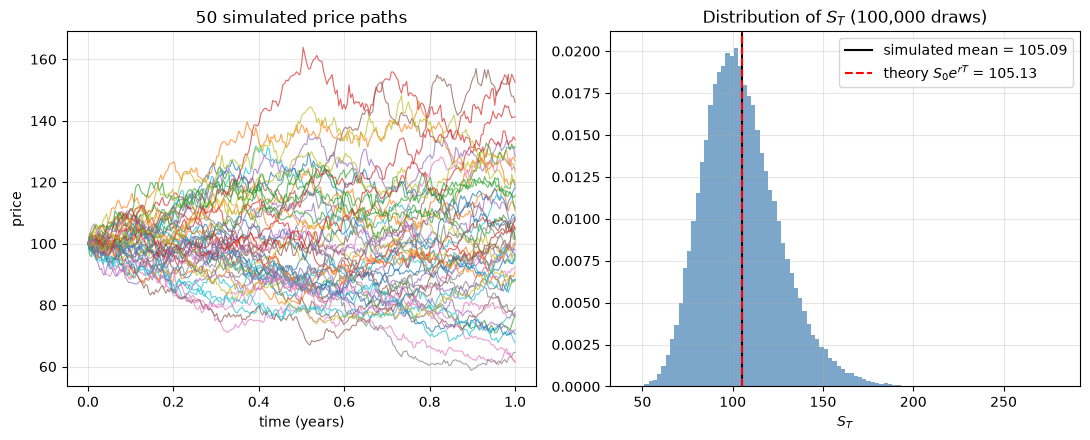
\includegraphics[width=\linewidth,height=3.7cm,keepaspectratio]{1_Monte_Carlo_Basics_4_0.png}
  \sourcecaption{Each path uses independent normal shocks}
\end{column}
\end{columns}
\end{frame}

% 5 -------------------------------------------------------------------------
\begin{frame}[fragile]{Monte Carlo estimator and confidence interval}
\small
\begin{columns}[T,onlytextwidth]
\begin{column}{0.48\textwidth}
  For $N$ simulated terminal prices, calculate each discounted payoff and take
  the sample average:
  \[
    \widehat V=e^{-rT}\frac1N\sum_{i=1}^{N}\text{payoff}(S_T^{(i)}).
  \]
  \begin{itemize}\setlength\itemsep{0.45em}
    \item The Law of Large Numbers makes $\widehat V$ converge to $V_0$.
    \item The CLT gives $\mathrm{SE}=\mathrm{sd}(\text{discounted payoff})/\sqrt N$.
    \item A 95\% interval is $\widehat V\pm1.96\,\mathrm{SE}$.
  \end{itemize}
\end{column}
\begin{column}{0.48\textwidth}
  \sourcecaption{The core simulation code used in our notebook}
  \begin{lstlisting}[language=Python,basicstyle=\ttfamily\tiny,breaklines=true,columns=flexible]
z = rng.standard_normal(N)
ST = s0 * np.exp((r - .5*sigma**2)*T
                 + sigma*np.sqrt(T)*z)
discounted = np.exp(-r*T) * payoff(ST, K, kind)
price = discounted.mean()
SE = discounted.std(ddof=1) / np.sqrt(N)
  \end{lstlisting}
\end{column}
\end{columns}
\end{frame}

% 6 -------------------------------------------------------------------------
\begin{frame}{Real-market study design}
\small
\begin{columns}[T,onlytextwidth]
\begin{column}{0.53\textwidth}
  \begin{block}{SPY option snapshot: 4 November 2026}
  \begin{tabular}{@{}lr@{}}
    Underlying price $S_0$ & \$754.35 \\
    Risk-free rate $r$ & 3.95\% \\
    60-day volatility $\sigma$ & 10.0\% \\
    Simulation size & 200,000 per expiry \\
    Final sample & 389 contracts
  \end{tabular}
  \end{block}
  \vspace{1mm}
  We keep strikes within $\pm10\%$ of $S_0$, require positive volume and
  recent trades, and discard options priced below \$0.10.
  \vspace{2mm}
  \textcolor{teal}{We compare Monte Carlo prices with market mid-prices, or last transactions when quotes are unavailable.}
\end{column}
\begin{column}{0.43\textwidth}
  \centering
  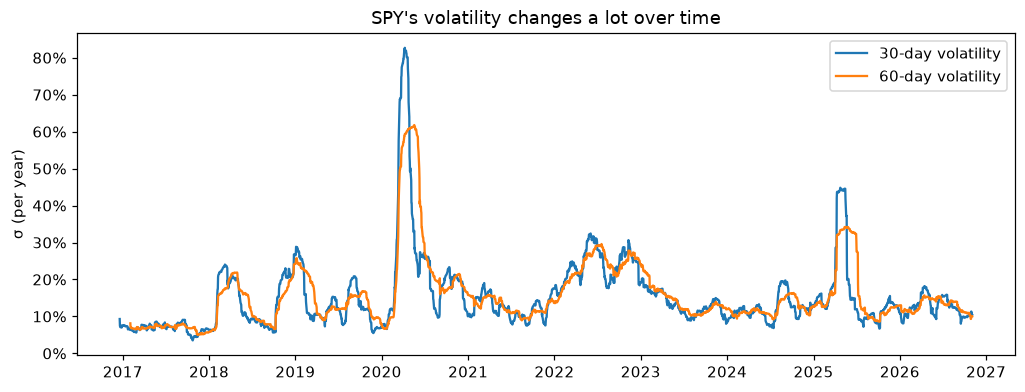
\includegraphics[width=\linewidth,height=4.0cm,keepaspectratio]{2_Market_Comparison_5_1.png}
  \sourcecaption{Notebook output: realised SPY volatility over time}
\end{column}
\end{columns}
\end{frame}

% 7 -------------------------------------------------------------------------
\begin{frame}{Validation against Black--Scholes}
\small
\begin{block}{Test case}
  $S_0=K=100$, $T=1$ year, $r=5\%$, $\sigma=20\%$, and 100,000 simulations.
\end{block}
\vspace{3mm}
\centering
\begin{tabular}{lrrrr}
\toprule
Option & Monte Carlo & 95\% confidence interval & Black--Scholes & Inside interval? \\
\midrule
Call & 10.44 & [10.35,\ 10.53] & 10.45 & Yes \\
Put  & 5.60  & [5.55,\ 5.66]  & 5.57  & Yes \\
\bottomrule
\end{tabular}
\vspace{7mm}
\begin{block}{Interpretation}
  The exact prices lie inside both confidence intervals. The small gaps are
  normal sampling variation, not an error in the pricing code.
\end{block}
\end{frame}

% 8 -------------------------------------------------------------------------
\begin{frame}{Monte Carlo error shrinks at the CLT rate}
\small
\begin{columns}[c,onlytextwidth]
\begin{column}{0.60\textwidth}
  \centering
  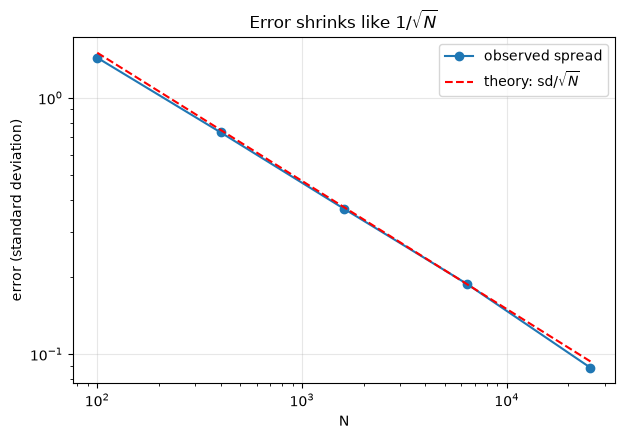
\includegraphics[width=\linewidth,height=5.25cm,keepaspectratio]{1_Monte_Carlo_Basics_12_0.png}
  \sourcecaption{Notebook output: 500 repeated estimates at each simulation size}
\end{column}
\begin{column}{0.36\textwidth}
  \begin{itemize}\setlength\itemsep{0.8em}
    \item Standard error is proportional to $1/\sqrt N$.
    \item Across 500 repeats, the observed spread closely follows theory.
    \item Increasing $N$ from 100 to 25,600 reduces the spread from 1.43 to 0.089.
  \end{itemize}
  \vspace{3mm}
  \textcolor{teal}{\textbf{Practical implication:} four times as many simulations only halve the error.}
\end{column}
\end{columns}
\end{frame}

% 9 -------------------------------------------------------------------------
\begin{frame}{Model price versus market price}
\small
\begin{columns}[T,onlytextwidth]
\begin{column}{0.59\textwidth}
  \centering
  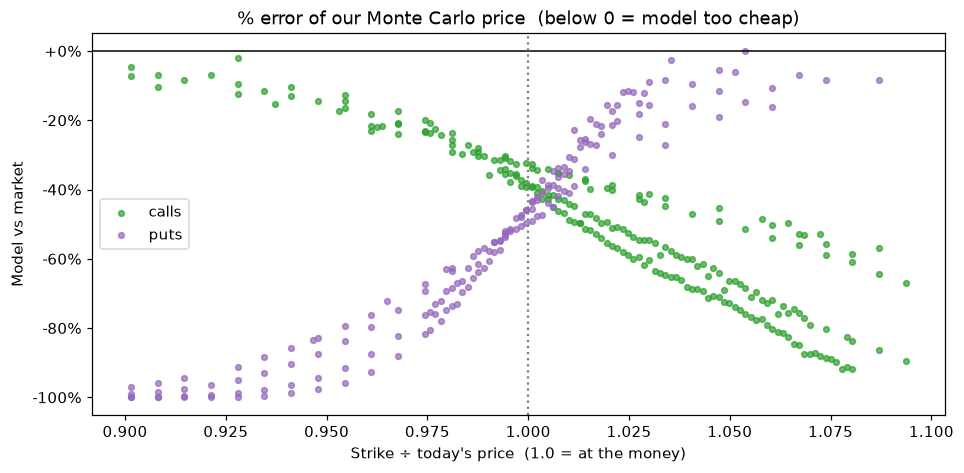
\includegraphics[width=\linewidth,height=5.1cm,keepaspectratio]{2_Market_Comparison_18_0.png}
  \sourcecaption{Notebook output: negative error means model price is below market price}
\end{column}
\begin{column}{0.37\textwidth}
  \textcolor{teal}{\textbf{Main result:} the model prices are below the market for almost every retained contract.}
  \vspace{2mm}
  \begin{itemize}\setlength\itemsep{0.6em}
    \item Near the money, prices are about 40\% lower, or roughly \$7.
    \item Monte Carlo matches Black--Scholes within \$0.12, with a typical 95\% margin of error of about $\pm\$0.05$.
  \end{itemize}
\end{column}
\end{columns}
\end{frame}

% 10 ------------------------------------------------------------------------
\begin{frame}{Volatility skew and conclusion}
\small
\begin{columns}[T,onlytextwidth]
\begin{column}{0.60\textwidth}
  \centering
  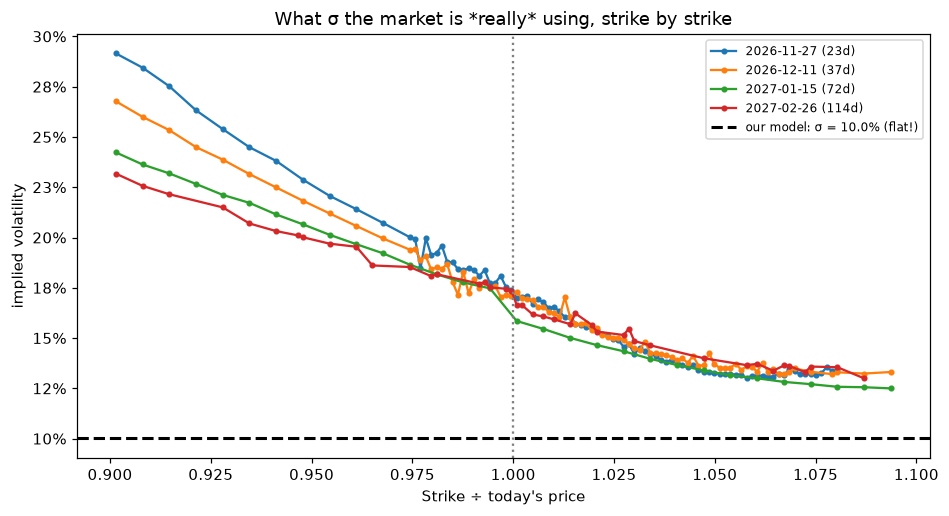
\includegraphics[width=\linewidth,height=4.65cm,keepaspectratio]{2_Market_Comparison_20_0.png}
  \sourcecaption{Notebook output: implied-volatility skew}
\end{column}
\begin{column}{0.36\textwidth}
  \begin{block}{What the market implies}
    \begin{tabular}{@{}lr@{}}
      60-day historical $\sigma$ & 10.0\% \\
      At-the-money implied $\sigma$ & 17.1\% \\
      90\% strike implied $\sigma$ & 24.8\% \\
      105--110\% strike implied $\sigma$ & 13.2\%
    \end{tabular}
  \end{block}
  \textbf{Conclusion.} Monte Carlo follows the LLN and CLT. The market gap reflects a weak volatility input: recent history misses future uncertainty and crash risk.
\end{column}
\end{columns}
\end{frame}

\end{document}
